\documentclass[]{scrartcl}
\usepackage{graphicx}
\usepackage{siunitx}
\usepackage{amsmath,amsthm,amssymb}
\usepackage[english]{babel}
\usepackage{hyperref}
\usepackage{booktabs}
\usepackage{subcaption}
\usepackage[backend=biber, style=numeric, safeinputenc, sorting=none]{biblatex}
\addbibresource{source.bib}

\title{Airborn sound isolation homework}
\date{Room Acoustics - Music and Acoustic Engineering -Politecnico di Milano}
\author{Lercari Mattia 10751919, Lampis Alessio 10743504}
\subtitle{01/11/2020 - Academic year 2020/2021}

\begin{document}
\maketitle

\section{Calculate the sound reduction index of each component}
\subsection{Facades}
The material that has been chosen to design facades of the room under study is lightweight concrete, $300$ mm  thick. The Sound Reduction Index (dB) are shown in Tab. \ref{tab:fac}. 
\begin{table}[h]
	\centering
	$\begin{array}{c|c|c|c|c|c|c}
	\toprule
	\SI{63}{\hertz} & \SI{125}{\hertz} & \SI{250}{\hertz} & \SI{500}{\hertz}  & \SI{1000}{\hertz} & \SI{2000}{\hertz} & \SI{4000}{\hertz} \\
	%\hline
	\midrule
	37 & 37 & 42 & 51 & 58 & 58 & 58 \\
	\bottomrule
	\end{array}$
	\caption{Octave-band values for the SRI of the facade walls.}
	\label{tab:fac}
\end{table} 
Since the values are given in octave bands, we need to interpolate them linearly to obtain a curve in 1/3-octave bands so that they are consistent with the reference curve. Linear interpolation is calculated using:
\begin{equation}
	R_f = R_{f1} + \frac{f - f_1}{f_2 - f_1}(R_{f2} - R_{f2}). \quad \quad  f_1<f<f_2
\end{equation} where $R_{fi} = R(f_i)$ indexes are referred to frequencies in  1/3-octave bands. The result can be found in \"Facade Wall" sheet. Moreover, its areic mass is $m'= 390 $ $ Kg/m^2$. From the table, as well as from the Excel computations, the weighted sound reduction index is $R_w = 54$ and correction coefficients $C$ and $C_{tr}$ are $-2$ and $-6$, respectively. 
\subsection{Windows}

\begin{figure}[h]
	\centering
	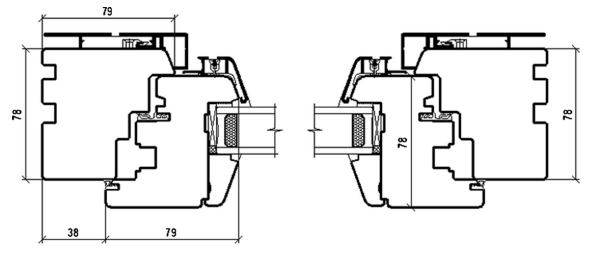
\includegraphics[width=0.7\linewidth]{windows_profile}
	\caption{Horizontal cross section of tested window}
	\label{fig:windowsprofile}
\end{figure}


The sound reduction indexes of the windows are taken from \cite{Window}. Here the authors report their measures of R in 1/3-octave bands from 100 Hz to 5000 Hz for different kinds of insulated glass units (IGUs) with double glass, all mounted in the same frame. These measurements are done in compliance with LST EN ISO 10140 series standards and the results were evaluated according to LST EN ISO 717-1 standard. For this homework we chose the IGU that is referred to  as WOG2/1 in the paper: it consists of two layers of ordinary glass\footnote{Ordinary" here stands for "not laminated", since other IGUs studied in the cited paper had one or both panes made out of laminated glass.} (4 mm and 6 mm of thickness respectively) with a 18 mm air gap filled with argon gas in between. Since the paper doesn't provide any information about material density, we used a common value of soda lime glass density, $ \rho = 2530$ $Kg/m^3$. The corresponding areic mass is $m' = 25.3$ $Kg/m^3$. 
The sound reduction index curve for WOG2/1 can be seen in Fig. \ref{fig:sri_win}. Based on these values we have computed $R_w$, $C$, and $C_{tr}$. Our value of $R_w = \SI{37}{\decibel}$ and the one given by the authors coincide, while the coefficients $C$ and $C_{tr}$ are $-2$ and $-6$ in our computation but $-1$ and $-5$ according to the cited study. 

\begin{figure}
	\centering
	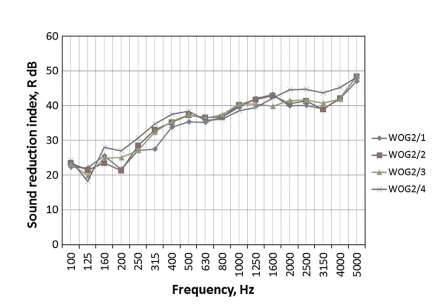
\includegraphics[width=0.7\linewidth]{windows_sound_reduction}
	\caption{Sound reduction index in 1/3-octave bands for different IGUs \cite{Window}. The curve we used in this homework is the one labeled WOG2/1.}
	\label{fig:sri_win}
\end{figure}


\subsection{Floor and ceiling}
Here too, we chose a material from the lecture slides: in particular, we chose the Ca-Si blocks ($240$ mm) as construction which has a remarkable areic mass ($420$ $Kg/m^2$). The sound reduction index values in octave bands are presented in Tab. \ref{tab:floor}.
\begin{table}[h]
	\centering
	$\begin{array}{c|c|c|c|c|c|c}
		\toprule
		\SI{63}{\hertz} & \SI{125}{\hertz} & \SI{250}{\hertz}  & \SI{500}{\hertz}  & \SI{1000}{\hertz}  & \SI{2000}{\hertz} & \SI{4000}{\hertz} \\
		\midrule
		38 & 38 & 46 & 54 & 62 & 68 & 68 \\
		\bottomrule
	\end{array}$
	\caption{Octave-band values for the SRI of the floor and ceiling.}
	\label{tab:floor}
\end{table}

The weighted value given by table is $56$ while it is $57$ in the Excel, as well as correction coefficients are $-1,-6$ in the table while $-2,-7$ in the sheets. 

\subsection{Internal walls}
From the catalogue of an italian company called FOROSON we found results of measurement realized on their bricks. We have considered walls made of FOROSON bricks with plaster, of total thickness equal to $33$ cm. The acoustic insulation properties were studied by the company according to UNI EN ISO 140-4 and $R_w'$ was computed following the UNI EN ISO 717-1. Since we used the same standards in our computations, our results for $R_w'$, $C$ and $C_{tr}$ are the same as those of the catalogue (see figure \ref{fig:poroton} ).
\begin{figure}[h]
	\centering
	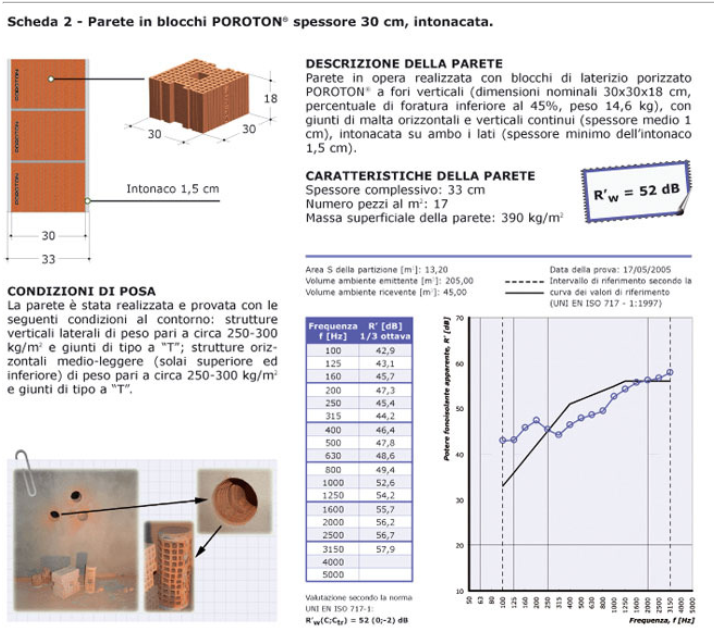
\includegraphics[width=0.9\linewidth]{poroton}
	\caption{Poroton results on plastered brick wall}
	\label{fig:poroton}
\end{figure}

\subsubsection{Door}
Since we wanted to have a wooden door while still keeping an high sound reduction index, we decided to use one made out of a particularly heavy wood, the ITIN (Prosopis kuntzei)\cite{wood}. Its density is $\mathit{1275 Kg/m^3}$ and we designed two layers of $\mathit{1 cm}$ of wood and a $\mathit{4 cm}$ of rockwool in between. Having these parameters and assuming a diffusive sound propagation through the door, we applied the mass law and obtained $R_w'= 40 dB (-4, -12)$. 

\section{Verify the passive acoustic requirements of buildings}  

In the Excel, section "data", are resumed sound absorption of each component between room A and room B given by direct and flanking contributions. In section "joints" are computed  vibration reduction index for each junction. The main result is the total weighted sound reduction index between room that is  $50,29$ $dB$, above the legal threshold of $50$ $dB$ (D.P.C.M 5-12-1997) as well as the facade sound reduction index, which is $53.3$ $dB$. 

\printbibliography

\end{document}
